\typeout{NT FILE state-of-the-art.tex}

\prependtographicspath{{Chapters/Figures/}}

\glsresetall

\chapter{State of the Art}
\label{cha:state-of-the-art}

In this chapter we'll explore how researchers have dealt with the challenges of creating an \gls{MAS} based \gls{CPPS}. We'll start by  examining the concepts of \gls{CPPS} and \gls{MAS} in more detail and by taking a look at the most commonly used designs and tools, as well as the recommended practices for an Industrial \gls{MAS}. Finally, we'll do a brief analysis on some prototypes that were made to showcase the usefulness of an MAS in an industrial setting.

\section{Cyber-Physical Production Systems}
\label{sec:cyber-physical_production_systems}

As stated before, a \Gls{CPS} is a system composed of two main entities, the physical system that contains all the hardware and resources and the cyber system that represents the physical system in the digital world. These two systems work together, the physical system sends data from the environment to the digital system and the digital system processes this data and instructs the physical system on what actions to perform. As such, this system works in a loop, constantly exchanging data and instructions to achieve a common goal.\\

A \Gls{CPPS} is, as the name implies, a \gls{CPS} that operates in a manufacturing setting. The physical system is composed of hardware like robot arms, \gls{AGV}s, conveyor belts and specialized machinery for manufacturing. The cyber system might be as simple as a computer program or as complex as a full-on three dimensional model of the physical system. \citeauthor{birgit01} \cite{birgit01} proposed that a \gls{CPPS} should:
\begin{itemize}
	\item Be service oriented, meaning that it should offer its services through the internet
	\item Be intelligent, with the ability to make decisions on its own
	\item Be interoperable, by having the capacity to aggregate and represent human-readable information and by providing a virtualization of the physical system
	\item Be able to flexibly adapt to changes in requirements and scale
	\item Have Big Data algorithm capable of processing data in real time
	\item Be capable of optimizing processes to increase \gls{OEE}
	\item Be able to integrate data across multiple disciplines and stages of the products life cycle
	\item Support secure communications to allow partnerships across companies
	\item Be capable of storing and accessing data in the Cloud
\end{itemize}

\section{Multi-Agent Systems}
\label{sec:multi-agent_systems}

\glsreset{MAS}

%If I need more content I can probably expand this section

% Industrial Agents {paulo02}
To understand what should be the best practices in an \gls{MAS} based \gls{CPPS}, we first need to understand its base characteristics. An \Gls{MAS} is, in essence a system composed by many entities called agents that have their own capabilities. These agents communicate and collaborate together by exchanging data among themselves and acting on that data to achieve a common goal. They are capable of adapting their behavior and of autonomous decision-making to determine the best course of action. This system is by nature decentralized and has no hierarchy, making it highly flexible and modular. At any point an agent can leave or join the system, without significant changes in architecture \cite{paulo02}.\\

% Recommendation of Best Practices for Industrial Agent Systems based on the IEEE 2660.1 Standard {Leitao2021};
Industrial agents inherit all the qualities of software agents, like the intelligence, autonomy and cooperation abilities, but in addition are also designed to operate in industrial settings, and need to satisfy certain industrial requirements such as reliability, scalability, resilience, manageability, maintainability and most important of all, hardware integration \cite{Leitao2021}. An example of a base architecture for an \gls{MAS} can be seen in Figure~\ref{fig:MAS_Architecture}. \\

\begin{figure}[h!]
	\centering
	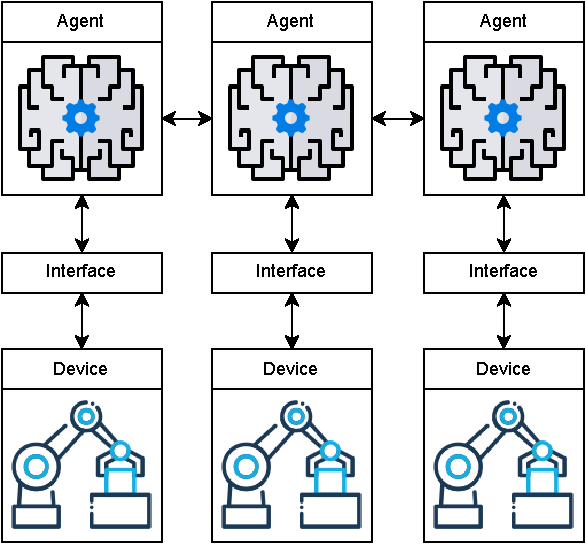
\includegraphics{MAS_Architecture}
	\caption{Industrial Multi-Agent System}
	\label{fig:MAS_Architecture}
\end{figure}

% Key directions for industrial agent based cyber-physical production systems {Karnouskos2019}
These requirements are generally tough to fulfill, especially so because despite the theoretical potential \gls{MAS} have shown in supporting them, there aren't a lot of agent-based production systems outside the prototyping phase. This has stopped the growth of Industrial \gls{MAS} due to the lack of practical knowledge in this field \cite{Karnouskos2019}. Another problem seen in Industrial \gls{MAS} is the lack of models that can represent these systems. One of the key elements of an \gls{MAS} are the changes made in structure and logic as the system operates. Thanks to the decentralized nature of the system, it is possible to add, remove or reconfigure modules freely to better adjust to the systems needs \cite{Karnouskos2019}.\\

Now that we have an idea of the characteristics and requirements for Industrial \gls{MAS}, we can take a look at the most commonly used architectures, followed by what is recommended by the IEEE Standard.

\subsection{Best Practices and Common Architectures}
\label{subsec:best_practices_and_common_architectures}

% Integration patterns for interfacing software agents with industrial automation systems {8591641}
% IEEE Recommended Practice for Industrial Agents: Integration of Software Agents and Low-Level Automation Functions {9340089}
\citeauthor{Leitao2021} \cite{Leitao2021} analyzed the IEEE 2660.1 Standard for the recommended practices in integrating software agents and low-level automation functions. They described the use of an MAS as a CPPS, where control is decentralized, emerging from the interactions of agents that are part of the system. And as we've discussed before, one of the biggest problems is creating an interface between the agent and the device associated with it. Because of this, the IEEE 2660.1 Standard was created, defining the best practices in designing one an appropriate interface.\\

As an example, the authors mention three main types of interfaces. An interface for a smart sensor, to acquire measurements. An interface for a \gls{PLC}, to control simple devices like conveyor systems. And finally, an interface for a robot controller to control more complex functions in the \gls{CPPS}. These three interfaces present different challenges on a development level, because each requires consideration on which architecture to follow, with different consequences to the evolution of the manufacturing plant over time.\\

The authors then created multiple scenarios, one of them being factory automation. They then proposed that the most valuable criterion was the response time of the system. As a secondary criterion scalability was chosen, but with a lesser importance. From this scenario the authors then concluded that a tightly coupled hybrid \gls{OPCUA} interface was preferable according to the IEEE 2660.1 standard. This means that the interface should have a client-server approach and be running remotely, a Tightly coupled Hybrid approach. However the authors also mention that this setup has a relatively low score, meaning that many of the other proposed practices are still viable, with testing needed to be done in order to pick the best one based on each specific scenario.\\


In \cite{Karnouskos2019}, it is proposed that one of the key requirements in the design of interfaces for \gls{MAS} is interoperability. This comes with other challenges associated, like re-usability and scalability. In an \gls{MAS}, the authors identified two main types of interfaces, the interface between agents, which normally is provided through the framework of the agent-based system, and the interface between agent and device. \\


\citeauthor{8591641} \cite{8591641} analyzed a study performed under the IEEE P2660.1 Working Group \cite{9340089} and concluded that most approaches followed a two-layer convention. The upper layer contained the agents part of the MAS and the lower layer the hardware associated with the physical production system. These two layers can interact in two ways \cite{8591641}:
\begin{itemize}
	\item Tight coupling, where the two layers communicate either through shared memory or through a direct network connection. This communication is synchronous and more direct.
	\item Loose coupling, where the two layers communicate through a queue or a pub/sub channel. This communication is asynchronous and less direct.
\end{itemize}

These layers can also be hosted in different setups \cite{8591641}:
\begin{itemize}
	\item Hybrid setup, where the two layers run in different devices.
	\item On-device setup, where the two layers run in the same device. 
\end{itemize}

This means that there can be four different interfaces, Tightly coupled Hybrid, Loosely coupled Hybrid, Tightly coupled On-device and Loosely coupled On-device.\\

A Tightly coupled Hybrid interface (Fig.~\ref{fig:tightly_coupled_hybrid}) is characterized by having the upper layer where the agent operates running remotely and accessing the lower layer through an \gls{API}. This \gls{API} is responsible for translating the instructions given by the agent into commands the hardware can interpret. It is also responsible for the opposite, translating the hardware output, such as error codes or function results into data the agent can use. This approach is limited by the channel through which both layers communicate since both agent and device operate on two different computing platforms. This channel is affected by the amount of traffic in the network, more connections implies a lesser quality of service, namely in response time \cite{8591641}.\\

\begin{figure}[h!]
	\centering
	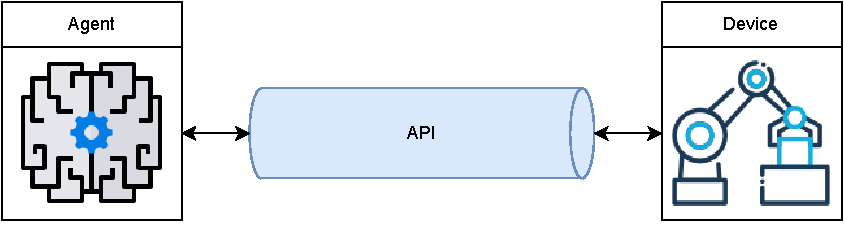
\includegraphics{TightlyCoupledHybrid}
	\caption{Tightly coupled Hybrid interface. Source: Adapted from \cite{8591641}}
	\label{fig:tightly_coupled_hybrid}
\end{figure}

A Loosely coupled Hybrid interface (Fig.~\ref{fig:loosely_coupled_hybrid}) also sees both agent and device running on different computing entities. The difference is that instead of each agent having a direct connection to the corresponding device, they communicate through a message broker. Since the system still runs on two different computers it still suffers from the quality of the connection between layers, making this somewhat inappropriate for systems highly dependent on real time action. However, this approach sees better results in complex systems, where the agent layer needs to publish information to a large amount of devices at once. It also sees good results when it comes to scaling the system, since both layers are very independent of each other \cite{8591641}.\\

\begin{figure}[h!]
	\centering
	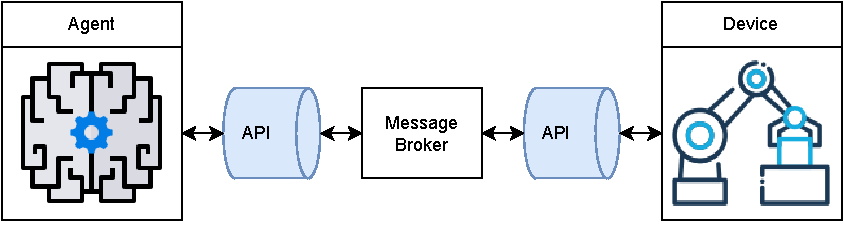
\includegraphics{LooselyCoupledHybrid}
	\caption{Loosely coupled Hybrid interface. Source: Adapted from \cite{8591641}}
	\label{fig:loosely_coupled_hybrid}
\end{figure}

A Tightly coupled On-device interface (Fig.~\ref{fig:tightly_coupled_ondevice}) on the other hand follows an architecture where both devices share the same physical platform and can be done in two different ways. The first one, and far less common, has both agent code and device code compiled into a single binary running in the same computing element. This solution provides far better results in very demanding real time applications, however it also removes some flexibility from the system and is far more complicated to design due to the lack of development tools. The second option has the computational resources shared through a software library, where communication is done through software functions but abstracting some elements. This option still holds good results in real time control, but not as good as the first one \cite{8591641}.\\\\

\begin{figure}[h!]
	\centering
	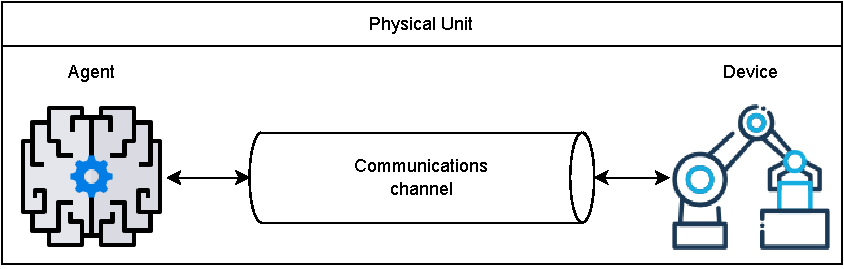
\includegraphics{TightlyCoupledOnDevice}
	\caption{Tightly coupled On-device interface. Source: Adapted from \cite{8591641}}
	\label{fig:tightly_coupled_ondevice}
\end{figure}

Finally, a Loosely coupled On-device interface (Fig.~\ref{fig:loosely_coupled_ondevice}) is characterized by having the agent embedded in the device and communication is done through a broker. Both layers share a physical unit but do not share computational resources. The utilization of a broker between the two layers offers some flexibility, since the agent and hardware are less dependent of each other. This comes with the caveat that the real time response of the whole unit is dependent on the performance of the broker \cite{8591641}.\\

\begin{figure}[h!]
	\centering
	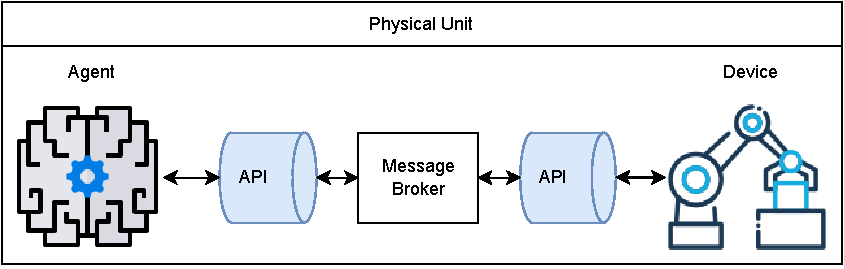
\includegraphics{LooselyCoupledOnDevice}
	\caption{Loosely coupled On-device interface. Source: Adapted from \cite{8591641}}
	\label{fig:loosely_coupled_ondevice}
\end{figure}

%Expand on JADE
The most common programming language to codify agents is Java, most likely due to JADE, an agent-based framework, followed by C++ \cite{8591641}. This framework helps developers in the implementation of \gls{MAS}s with the \gls{FIPA} specifications. It also allows deployment for different machines, due to Java supporting multiple devices \cite{JADE_website}.
For the device part, preexisting hardware is used in the majority of cases because it can be integrated into an \gls{MAS} by using protocols such as \gls{OPCUA} \cite{8591641}, which is a platform independent data exchange standard. It allows for both server-client and publish/subscribe communications as well see in Section~\ref{subsec:opcua} \cite{OPCUA_website}.

\subsection{OPC UA}
\label{subsec:opcua}

\glsreset{OPCUA}

% Explain OPC UA, maybe change the location of this subsection in the text to give more context to other subsections?

Another way to integrate hardware into an \gls{MAS} it through the use of already made libraries. \gls{OPCUA} was created based on \gls{OPC}, which in turn is based on the \gls{COMDCOM} for the exchange of data. \gls{OPCUA} is an evolution of \gls{OPC} but with extra functionalities, like added security, extensibility and platform independence. This last feature allowed it to run on many more platforms such as cloud-based servers, micro-controllers and \gls{PLC}s \cite{OPCUA_website}. As mentioned in Section~\ref{subsec:best_practices_and_common_architectures}, it is a recommended way to implement an interface for an \gls{MAS}. \gls{OPCUA} can be used with as a tightly coupled or loosely coupled interface, because it supports both direct client-server connections and pub/sub message transmissions, making it a strong option to integrate hardware into an \gls{MAS}.\\

Because \gls{OPCUA} already implements communication protocols and communication infrastructure, as well as an information model, all participants in the network know how to communicate. This means that the \gls{MAS} can be running on any kind of platform or be programmed in any kind of language, increasing system flexibility. Many modern \gls{PLC}s already provide an embedded \gls{OPCUA} server facilitating their integration into a new system \cite{Seitz2021}.

\subsection{Modbus}

Another way to integrate hardware into an \gls{MAS} is by using Modbus. Modbus is an industrial communications system that has been around since 1979. It follows a master/slave architecture, where the master is usually an application capable of acquiring data and the slave a \gls{PLC}. This master application can be substituted for an agent from an \gls{MAS}, integrating it with the slave hardware. Modbus supports standard \gls{TCPIP} and \gls{UDP}. It is simple, has high levels of compatibility and is decentralized due to the use of master/slave communications, making it flexible. Modbus could be integrated with any programming language of choice, by using software libraries to interpret and send commands to the Modbus layer \cite{10084891}.
% analysis on the specific interface implementations?
% I can probably analyze MAS with other objectives in mind to compare them to Industrial Agents?
\section{Practical Uses}
\label{sec:practical_uses}

Adoption of industrial oriented \gls{MAS} has been slow. According to \citeauthor{karnouskos02} \cite{karnouskos02}, the technology was still in its infancy almost two decades ago, with an incremental progress at best being made since then. In \cite{Karnouskos2019}, \citeauthor{Karnouskos2019} claim that agent-based applications in the industry is still limited. This is because despite the potential shown, these systems have not been implemented in real-world applications, where they would have the chance to evolve and leave the prototyping phase as new research is being done to make them more suitable for these applications.\\

There are, although, many research prototypes of \gls{MAS} used for an industrial applications, and we'll take a look at some of them in this section.

\subsection{Bottling Plant}
\label{subsec:bottling_plant}

For the design of the bottling plant in \cite{bottling_plant_part2}, a research paper \cite{bottling_plant_part1} was first done by \citeauthor{bottling_plant_part1}, with the collaboration of multiple partners from different backgrounds. This was done to define the base requirements for the \gls{CPPS} as well as the associated \gls{MAS}. These requirements are:

\begin{itemize}
	\item Easy Scalability and Functional Expansion
	\item Manufacturer-neutral Resource Representation
	\item Robust Production Control by the Product
	\item Lot Size One without Identification
\end{itemize}

Summarizing, the system needed to be easily scalable and it must be able to expand its functions to handle changes in production, it must be able to represent the resources in the \gls{CPPS} as a generic and manufacturer independent representation, products must be able to handle their own production steps, handling errors and reacting robustly to those errors and finally be able to produce lot sizes of one without needing an identification system for each individual product.\\

In consequence of these requirements, \citeauthor{bottling_plant_part1} designed a base solution consisting of two generic agents, a \gls{PA} that represents individual products being manufactured, in this case the beverage bottles, and a \gls{RA} that represents the resources used to manufacture the beverage bottles.\\

The \gls{MAS} was made using JADE, and as such all agents in this system are \gls{FIPA} compliant and communicate through \gls{FIPA} Requests and the \gls{FIPA} Contract Net.\\

Each agent inherits from a generic class called Agent. The \gls{RA} and \gls{PA} then inherit from this class, with added functionalities and variable fields. The \gls{PA} is an agent with the capabilities of performing autonomous and goal-driven behaviors. The \gls{RA} is an agent capable of controlling the physical resources by using sensor data and messages with hardware instructions.\\

A \gls{PA} differs from the generic Agent by implementing a configuration file ProductConfig. This file is in the \gls{XML} format and has information on the product represented by it. It also has a PlanningModule, which is essentially a StateMachine with all the products processing instructions.\\

Like the \gls{PA}, the \gls{RA} also mirrors the Agent class. It must be generic in order to be implemented on multiple resources, so for each ResourceType there exists a ResourceConfig file which is loaded onto the \gls{RA} in order to implement its interface. To give an example, if the resource has the ResourceType Machine, the ResourceConfig file MachineConfig must be loaded.

The authors identified five different ResourceTypes by classifying many resources from renowned machine manufacturers. \gls{RA}s not only include robots, transport systems and stations but also databases, as a data acquisition method. The authors recognize that not all types of possible resources for a \gls{CPPS} have been considered. This means that for every new resource type that needs to be added to the system, a new ResourceConfig must be created in order to integrate the new \gls{RA} into the system. In addition, a new resource that communicates differently from the ones already in the system would need a new interface, and thus a new ResourceConfig would also need to be created, even if the new resource performs similar functions in the manufacturing plant.\\

In \cite{bottling_plant_part2}, \citeauthor{bottling_plant_part2} created the service oriented bottling plant using the industrial agent system designed in \cite{bottling_plant_part1}, with positive results. To allow for extensibility of the system by additional resources a new agent class was created called \gls{IntA}. The ResourceConfig files for each type of \gls{RA} now have a new field which contains an InterfaceAgentConfig. This new \gls{IntA} is instantiated by the \gls{RA}s following the configurations of their respective InterfaceAgentConfig and it extends either a DBLinkAgent, used to connect to a database, and a PLCLinkAgent, used to connect to a \gls{OPCUA} client. All the information, like server address, port and authentication, is stored in the InterfaceAgentConfig file. By using \gls{OPCUA}, the system can now interface with the hardware in the manufacturing plant, through a Loosely Coupled Hybrid interface. The authors recognize that according to the IEEE P2660.1 Working Group the scalability is considered weak, although they claim the flexibility is worth this loss in scalability.\\

To implement a new \gls{IntA}, the following must be provided:
\begin{itemize}
	\item The communications protocol and the address, ports and authentication
	\item The way the interactions between the agent and resource should proceed
	\item The rules for the interpretation of internal resource states
\end{itemize}

Communication between the PLCLinkAgent and the machine is done through the use of simple commands. They specify the command to perform and the program type to use and must also include a unique name, the NodeID which identifies the type of the given input on the \gls{OPCUA} server, the data type, all possible values, the read/write direction and the description. The program type is chosen based on the size of the bottle and the command has to be one of the five commands already defined:

\begin{itemize}
	\item NoCommand, in case no action is needed
	\item ProductInPosition, in case the product is in position and ready
	\item ExecuteProcess, in case the process should start
	\item ProductRemoved, in case the product needs to be removed from the machine/station
	\item PrepareMachine, in case the machine needs to be prepared for a process to start
\end{itemize}

All commands have a number code associated to them to facilitate communications and at any time the PLCLinkAgent can retrieve the state of a machine by observing a NodeID with the machine state code. In Figure~\ref{fig:bottling_plant_state_achine} we can see the state machine representing the interactions between the PLCLinkAgent and a machine. To handle manufacturer specific machine state codes, the authors mapped said codes onto generic \gls{MAS} states, with the possibility of having multiple codes mapped to a single state. This was done to make the system capable of handling machines from different manufacturers without sacrificing flexibility in the \gls{MAS}.

\begin{figure}[h!]
	\centering
	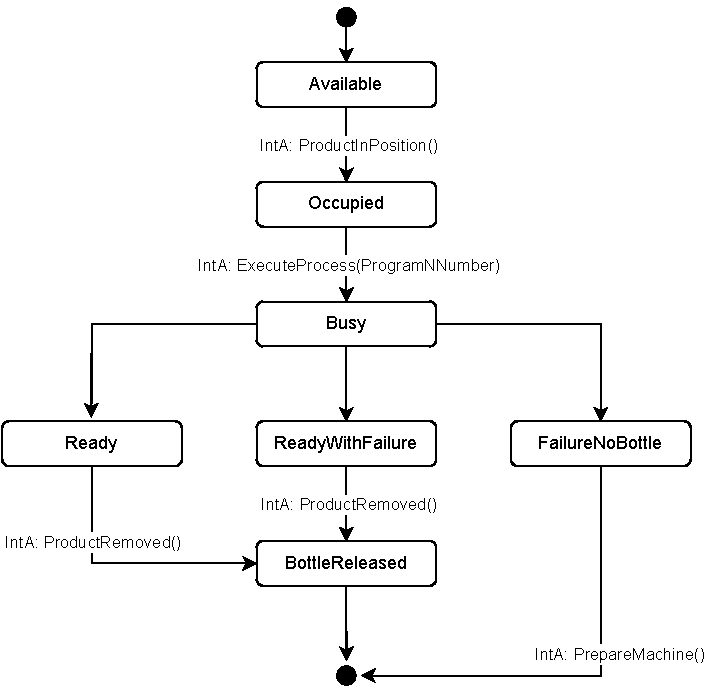
\includegraphics{BottlingPlantStateMachine}
	\caption{Interactions between PLCLinkAgent and \gls{PLC}. Source: Adapted from \cite{bottling_plant_part2}}
	\label{fig:bottling_plant_state_achine}
\end{figure}

The use of \gls{OPCUA} makes this system very flexible. New hardware that needs to be implemented in the system can be configured to use these commands through the use of a \gls{PLC}. The use of generic states make it scalable and configuration files also help fulfilling this necessity. However, it is still dependent on these files, with individual configurations needed for different manufacturers and machine types. The system also needs to be adapted to recognize the machine states from the new implemented hardware.

Nevertheless this system performed as intended, producing customized beverage bottles according the customers specifications. It is a good example of an \gls{MAS} based \gls{CPPS}, flexible, scalable, robust, with decentralized control and autonomous intelligent agents.
 
\subsection{Agent-based Plug and Produce CPPS}
\label{agent_plug_and_produce}

\citeauthor{8972169} \cite{8972169} have created a Plug and Produce \gls{CPPS}. It is capable of integrating new agents on the fly, as the system operates. First, the authors divided the system into three layers. The upper layer is where the \gls{MAS} operates, called the fog layer. The middle layer is where the interface between the \gls{MAS} and the hardware is, called the edge layer. And finally, the lower layer is where the hardware components of the \gls{CPPS} are, called the physical layer.\\

\glsreset{PA}
\glsreset{RA}

The agents were also categorized into \gls{PA} and \gls{RA}, performing similar functions to the ones in Section~\ref{subsec:bottling_plant} and in addition the authors also considered \gls{TA}s which abstract all resources whose function is to move a product from point A to point B. They also considered a \gls{DA} tasked with managing the existence of all other agents. This \gls{DA} should create a new agent or remove an existing one whenever a physical resource is plugged into or unplugged from the system.\\

To accomplish this the authors considered the grouping of a physical resource with its agent a Module. Modules are the components of the whole production system, and they can be plugged and unplugged at any time. The system need to be able to operate to the best of its abilities at all times. In Figure~\ref{fig:plug_and_play_device_architecture} we can see an example of one of these Modules.\\

\begin{figure}[h!]
	\centering
	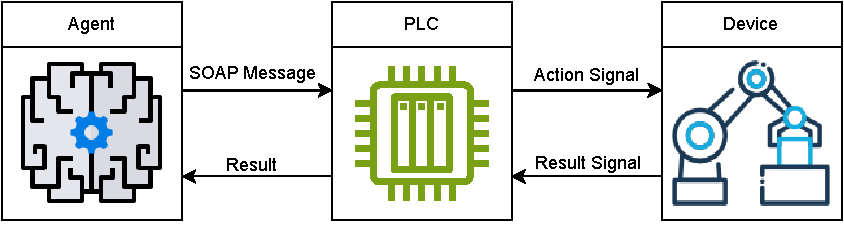
\includegraphics{PlugAndPlayDiagram}
	\caption{Plug and Produce \gls{RA}. Source: Adapted from \cite{8972169}}
	\label{fig:plug_and_play_device_architecture}
\end{figure}

For the interface between hardware and agent, \gls{PLC}s were chosen. These \gls{PLC}s are able to communicate using \gls{DWPS}. For the \gls{DA}, a Java class was implemented using the \gls{WS4D-JMEDS} framework, which searched for the devices in the network and obtained information about them. It was able to detect all devices connected to the network and add and remove them as needed.\\

Each resource is able to perform certain procedures on the products, represented in the \gls{MAS} as skill which \gls{RA}s perform on to \gls{PA}s. This is how the authors simulate the system virtually, whenever a product needs a certain procedure to be performed on itself, the corresponding \gls{PA} asks an \gls{RA} for that skill. This is relevant because the system may or may not have a resource able to perform a specific skill. In the case of a \gls{PA} that needs an non-existing skill to be performed, it waits until an \gls{RA} capable of performing the needed skill to be plugged into the system.\\

The \gls{MAS} was developed in the JADE framework, all agents are therefore \gls{FIPA} compliant and communicate through \gls{FIPA} Requests and \gls{FIPA} Contract Net. More precisely, the \gls{FIPA} Requests are used for \gls{PA}-\gls{TA} communications and the \gls{FIPA} Contract Net used for \gls{PA}-\gls{RA} communications. Whenever a new \gls{PA} enters the system, it asks through the \gls{FIPA} Contract Net which \gls{RA}s are can perform the needed skill. After getting responses from all the \gls{RA}s, the \gls{PA} picks the best one and receives its location. It then sends a \gls{FIPA} Request to the \gls{TA} to transport it to this location. After arriving, it then requests that the skill be performed to the \gls{RA}.\\

This system was used to simulate a simple conveyor belt line with brushing capabilities. The authors where able to successfully plug and unplugged Modules from the system during its operation. The \gls{DA} correctly connected and disconnected hardware components from the system and deployed and kicked agents from the system accordingly. This shows that an \gls{MAS} built from the ground up with these functionalities is very powerful in its scalability, and although this was only a prototype it shows a lot of promise for a dynamic system.

\subsection{PRIME}

\citeauthor{PRIME_plug_and_produce} \cite{PRIME_plug_and_produce} have done a demonstration on the PRIME architecture as an agent based framework with plug and produce functionalities. PRIME is a project developed thanks to the European FP7 program, and it proposes a solution to allow plug and produce using any kind of computational devices. This means that it is no longer needed to restrict a manufacturing plant to specific controllers to provide to it some sort of reconfigurability and flexibility. It allows any kind of controller or to be integrated into the system while still using the same framework.\\

All agents in this framework were developed using JADE, therefore all agents are \gls{FIPA} compliant. This adds to the plug and produce functionality of the system. The PRIME agent system is composed of eight different agents:
\begin{itemize}
	\item \gls{PSA} is the highest level agent in the framework. It manages the current state of the system.
	\item \gls{PMA} is responsible to combine all resources and tasks in the same space to abstract certain functionalities
	\item \gls{SMA} works in tandem with a \gls{PMA}, combining the lower-level skills into higher-level ones according to pre-defined rules, that the associated \gls{PMA} then provides to the system
	\item \gls{CA} is the agent that abstracts the hardware in the \gls{CPPS}. It is able to read and write data to and from the hardware
	\item Local Monitoring and Data Analyses
\end{itemize}

All devices to be integrated into the system were categorized into three groups according to their characteristics:
\begin{itemize}
	\item Fully intelligent resources, capable of running the necessary agents locally, typically a machine with the ability to run the Java environment, setup in a Tightly or Loosely Coupled On-device architecture
	\item Semi-intelligent resources, capable of announcing their existence to the system and of reconfiguring themselves but without the ability to run the Java environment, setup in a Tightly or Loosely Coupled hybrid architecture
	\item Passive resources, without any computational abilities and dependent on a controller to connect them to the main system  
\end{itemize}

For the first type of device, PRIME was able to very easily connect to it. The device ran all the necessary components to enable communications and to expose itself to the network. It ran the necessary agents related to the hardware locally and the main framework was able to configure the hardware by interacting with the local agents, which in turn interfaced with the device. This is the type of architecture preferred by PRIME, since it provides all services autonomously \cite{PRIME_plug_and_produce}.\\

For second category of devices an INICO \gls{PLC} capable of running \gls{DWPS} was needed to connect the device to the framework since they can't run the agents locally. An auxiliary computer running the \gls{DWPS} software was responsible for detecting the \gls{PLC} and connecting to it. The necessary agents running on this computer launched the hardware related agents whenever they detected a new device running \gls{DWPS}, and these local agents were able to connect to the main PRIME network \cite{PRIME_plug_and_produce}.\\

The last category of devices is the most complicated one because they have no easy way to interface with the main system. In this case a more primitive \gls{PLC} was used to simulate this limitation. An auxiliary computer running the JADE framework with all necessary agents is needed to create this interface and the system communicates with the \gls{PLC} on a case-by-case scenario, with each \gls{PLC} possibly needing different configurations. When the relevant agent detect a new device, it launches a new agent to interface with this device. The new agent then uses a case specific library to interface the \gls{PLC} using standard protocols \cite{PRIME_plug_and_produce}. This last option is not flexible and uses a case-by-case configuration, making it the least desirable in a system.
